\documentclass[12pt, a4paper, oneside]{ctexart}
\usepackage[backend=biber]{biblatex}
\usepackage{amsmath, amsthm, amssymb, appendix, bm, graphicx, hyperref, mathrsfs,adjustbox,enumerate,colortbl,bbding,booktabs,subcaption,algorithm, algorithmic}
\usepackage[table]{xcolor}
\addbibresource{biber.bib}
\title{\textbf{论文标题}}
\author{tanghongyu}
\date{\today}
\linespread{1.5}
\newtheorem{theorem}{定理}[section]
\newtheorem{definition}[theorem]{定义}
\newtheorem{lemma}[theorem]{引理}
\newtheorem{corollary}[theorem]{推论}
\newtheorem{example}[theorem]{例}
\newtheorem{proposition}[theorem]{命题}
\renewcommand{\abstractname}{\Large\textbf{摘要}}

\definecolor{blue}{RGB}{125,176,220}
\definecolor{dark_green}{RGB}{81,178,103}
\definecolor{light_green}{RGB}{202,224,173}
\definecolor{yellow}{RGB}{246,239,96}


\begin{document}

\maketitle

\setcounter{page}{0}
\maketitle
\thispagestyle{empty}
\newpage
\begin{abstract}
    这里是摘要。这里是摘要。这里是摘要。这里是摘要。这里是摘要。这里是摘要。这里是摘要。这里是摘要。这里是摘要。这里是摘要。这里是摘要。这里是摘要。
    \par\textbf{关键词:}这里是关键词; 这里是关键词。
\end{abstract}

\newpage
\pagenumbering{Roman}
\setcounter{page}{1}
\tableofcontents
\newpage
\setcounter{page}{1}
\pagenumbering{arabic}

\section{定理}

%\subsection{二级标题}
dingli\cite{elgamal1985public}
\newpage




\section{表格}

\begin{table}[htbp]
    \centering  % 显示位置为中间
    \caption{ }  % 表格标题
    \label{tab1}  % 用于索引表格的标签
    %字母的个数对应列数,|代表分割线
    % l代表左对齐,c代表居中,r代表右对齐
    \begin{tabular}{|c|c|c|}
    \end{tabular}
\end{table}
%\begin{theorem}

%\end{theorem}

\begin{table}[htbp]
    \centering  % 显示位置为中间
    \caption{ }  % 表格标题
    \label{tab2}  % 用于索引表格的标签
    %字母的个数对应列数,|代表分割线
    % l代表左对齐,c代表居中,r代表右对齐
    \begin{adjustbox}{max width=\textwidth}
        \begin{tabular}{|c|c|c|}
        \end{tabular}
    \end{adjustbox}
\end{table}



\begin{itemize}
    \item \colorbox{blue}{blue}
    \item \colorbox{dark_green}{dark green}
    \item \colorbox{light_green}{light green}
    \item \colorbox{yellow}{yellow}
\end{itemize}


\begin{table}[htbp]
    \centering
    \begin{tabular}{cccc}
        \toprule
        \textbf{蓝色}                      & \textbf{浅绿色}                            & \textbf{深绿色}                           & \textbf{黄色}                        \\
        \midrule
        \cellcolor{blue}\footnotemark[1] & \cellcolor{light_green}\footnotemark[2] & \cellcolor{dark_green}\footnotemark[3] & \cellcolor{yellow}\footnotemark[4] \\
        \bottomrule
    \end{tabular}
\end{table}
\footnotetext[1]{这是蓝色}
\footnotetext[2]{这是深绿色}
\footnotetext[3]{这是浅蓝色}
\footnotetext[4]{这是黄色}

\newpage

\section{图片}
\subsection{单图}
\begin{figure*} [htbp!]
    \makebox[\textwidth][c]{\includegraphics[width=1.2\textwidth]{fig/chiji.png}}%使用此代码需注意图片比例,否则图片会被伸缩
    %\includegraphics[scale=0.25]{chiji.png}%按比例缩放的时候可以用次代码

    \caption{0杀吃鸡}
    \label{fig1}
\end{figure*}
\subsection{多图}

\begin{figure}[htbp]
    \centering
    \begin{subfigure}{0.3\textwidth}
        \centering
        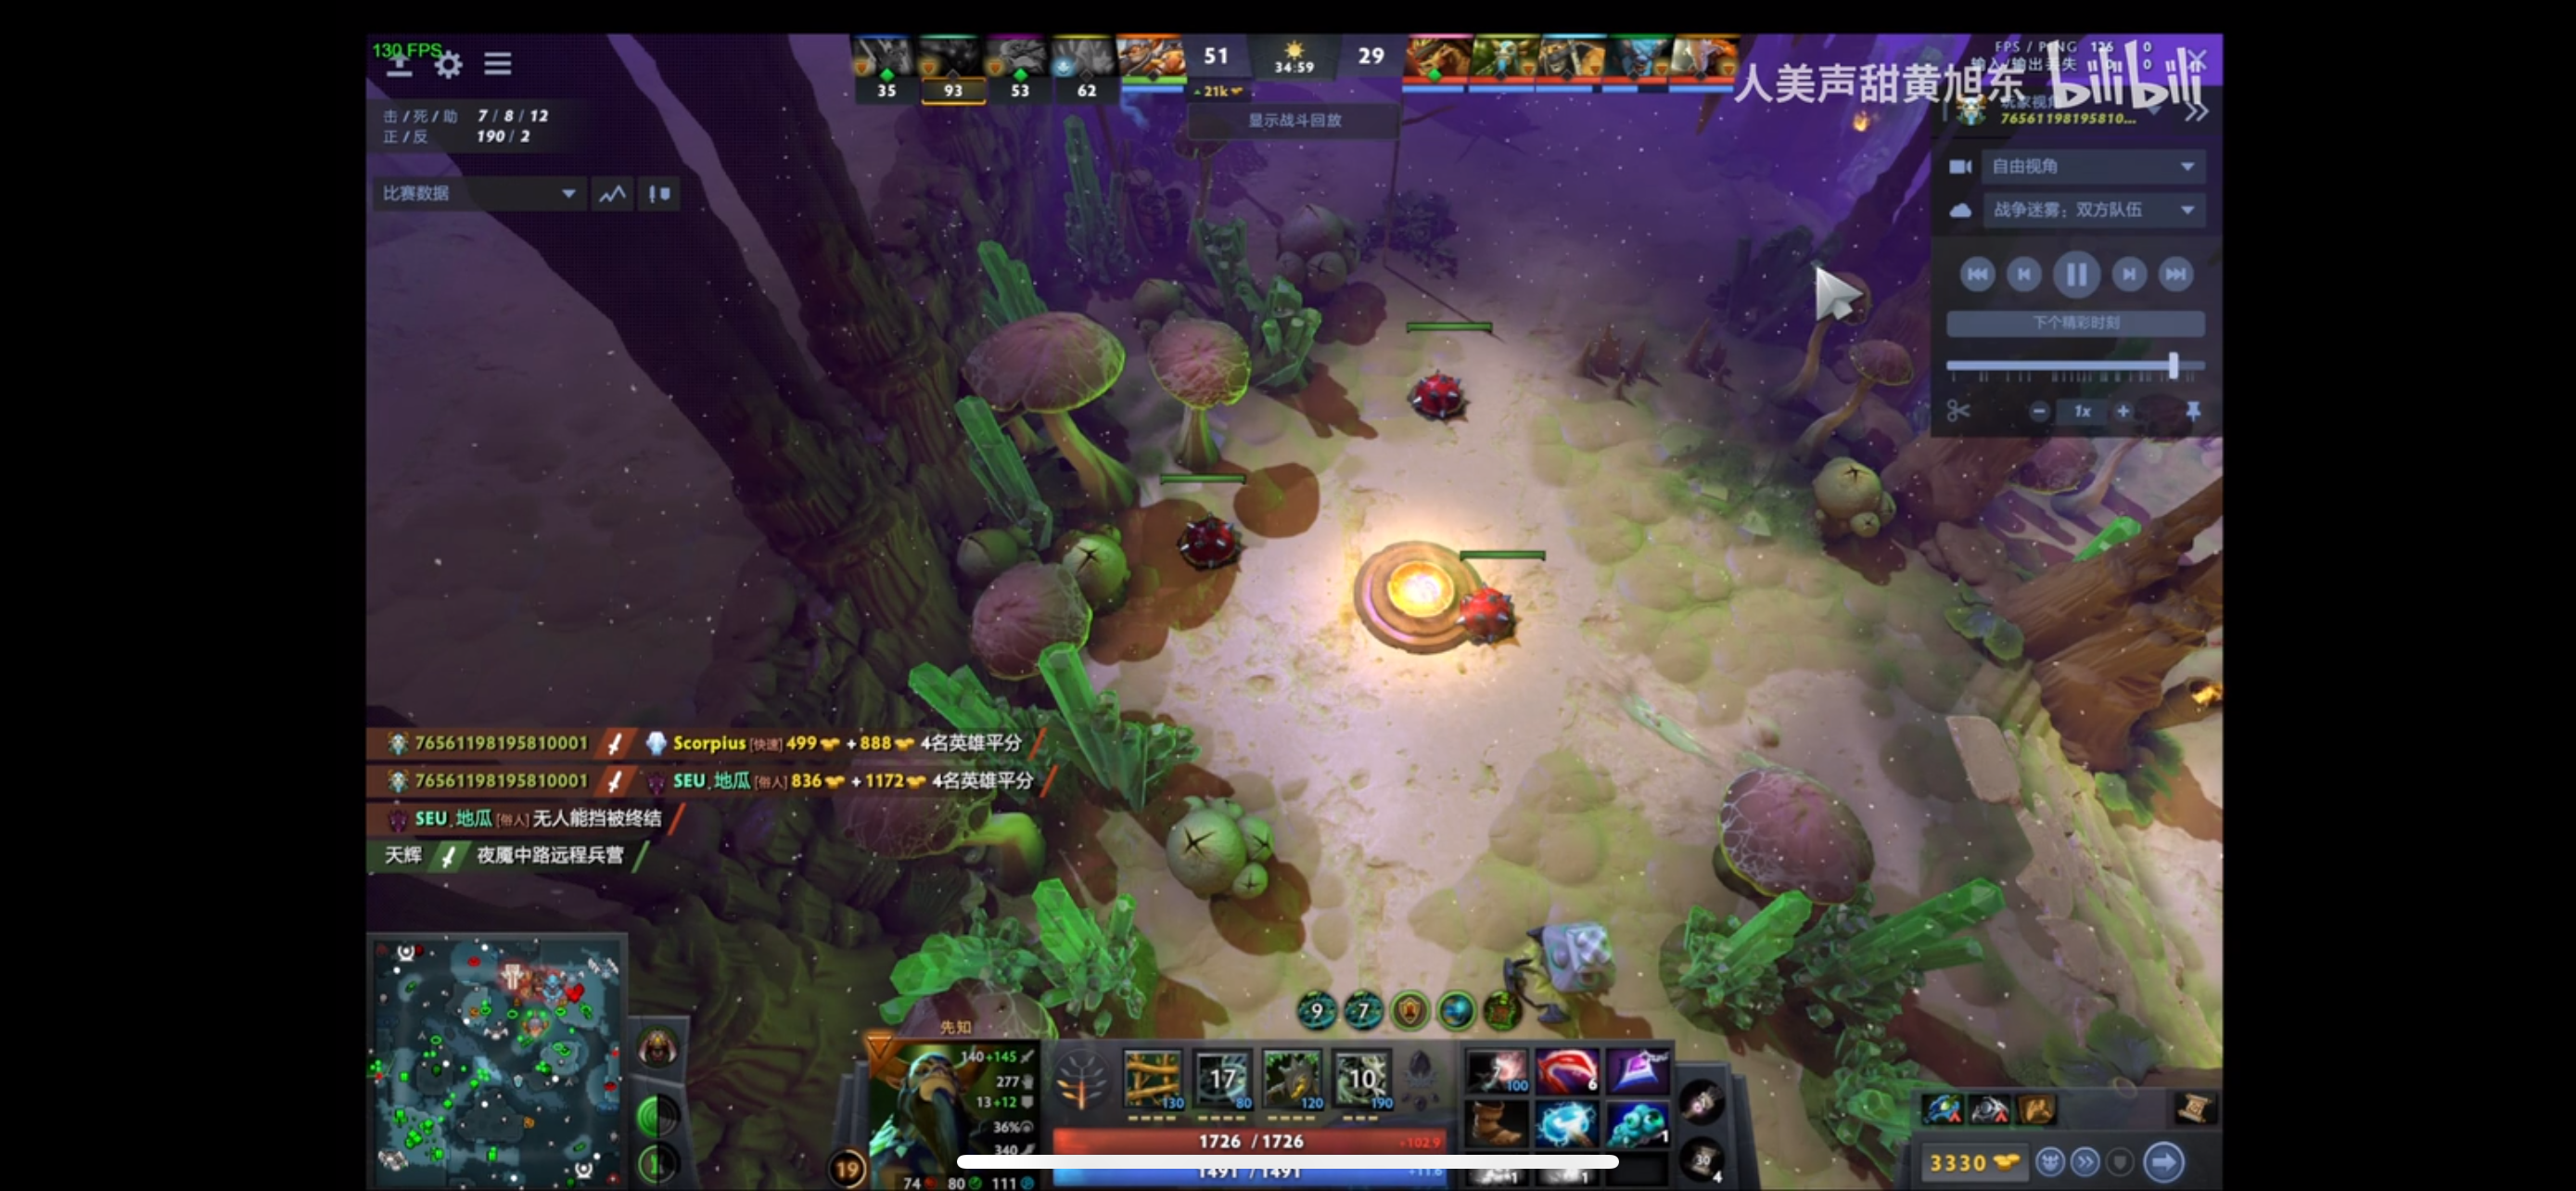
\includegraphics[width=\textwidth]{fig/1.png} % 图片1
        \caption{图1}
    \end{subfigure}
    \hfill
    \begin{subfigure}{0.3\textwidth}
        \centering
        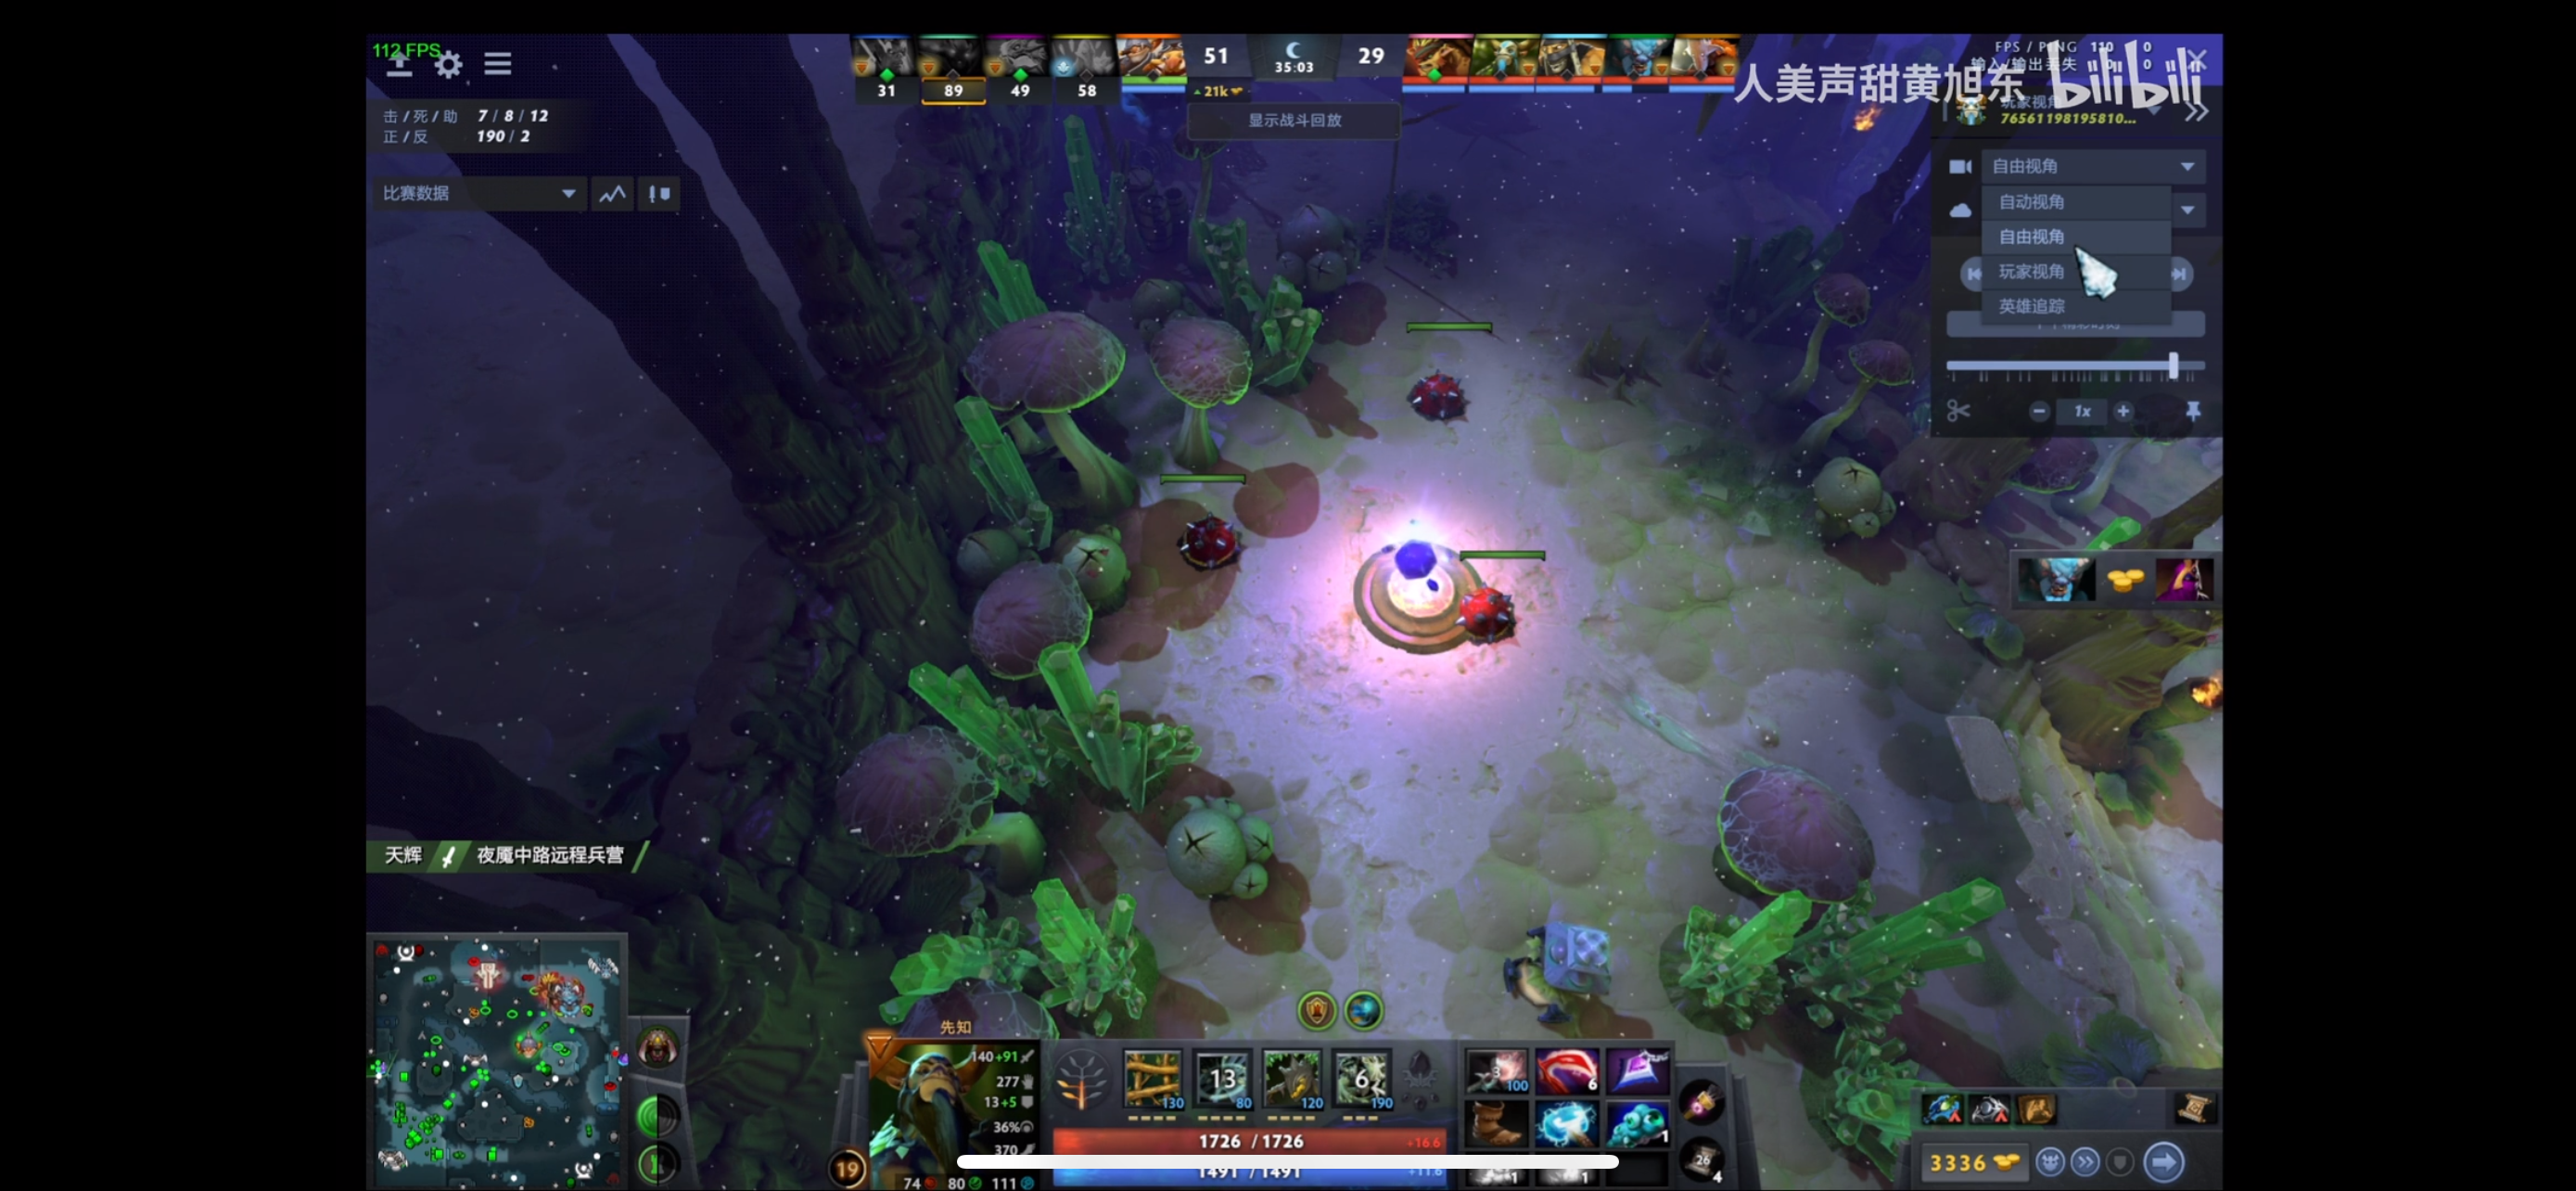
\includegraphics[width=\textwidth]{fig/2.png} % 图片2
        \caption{图2}
    \end{subfigure}
    \hfill
    \begin{subfigure}{0.3\textwidth}
        \centering
        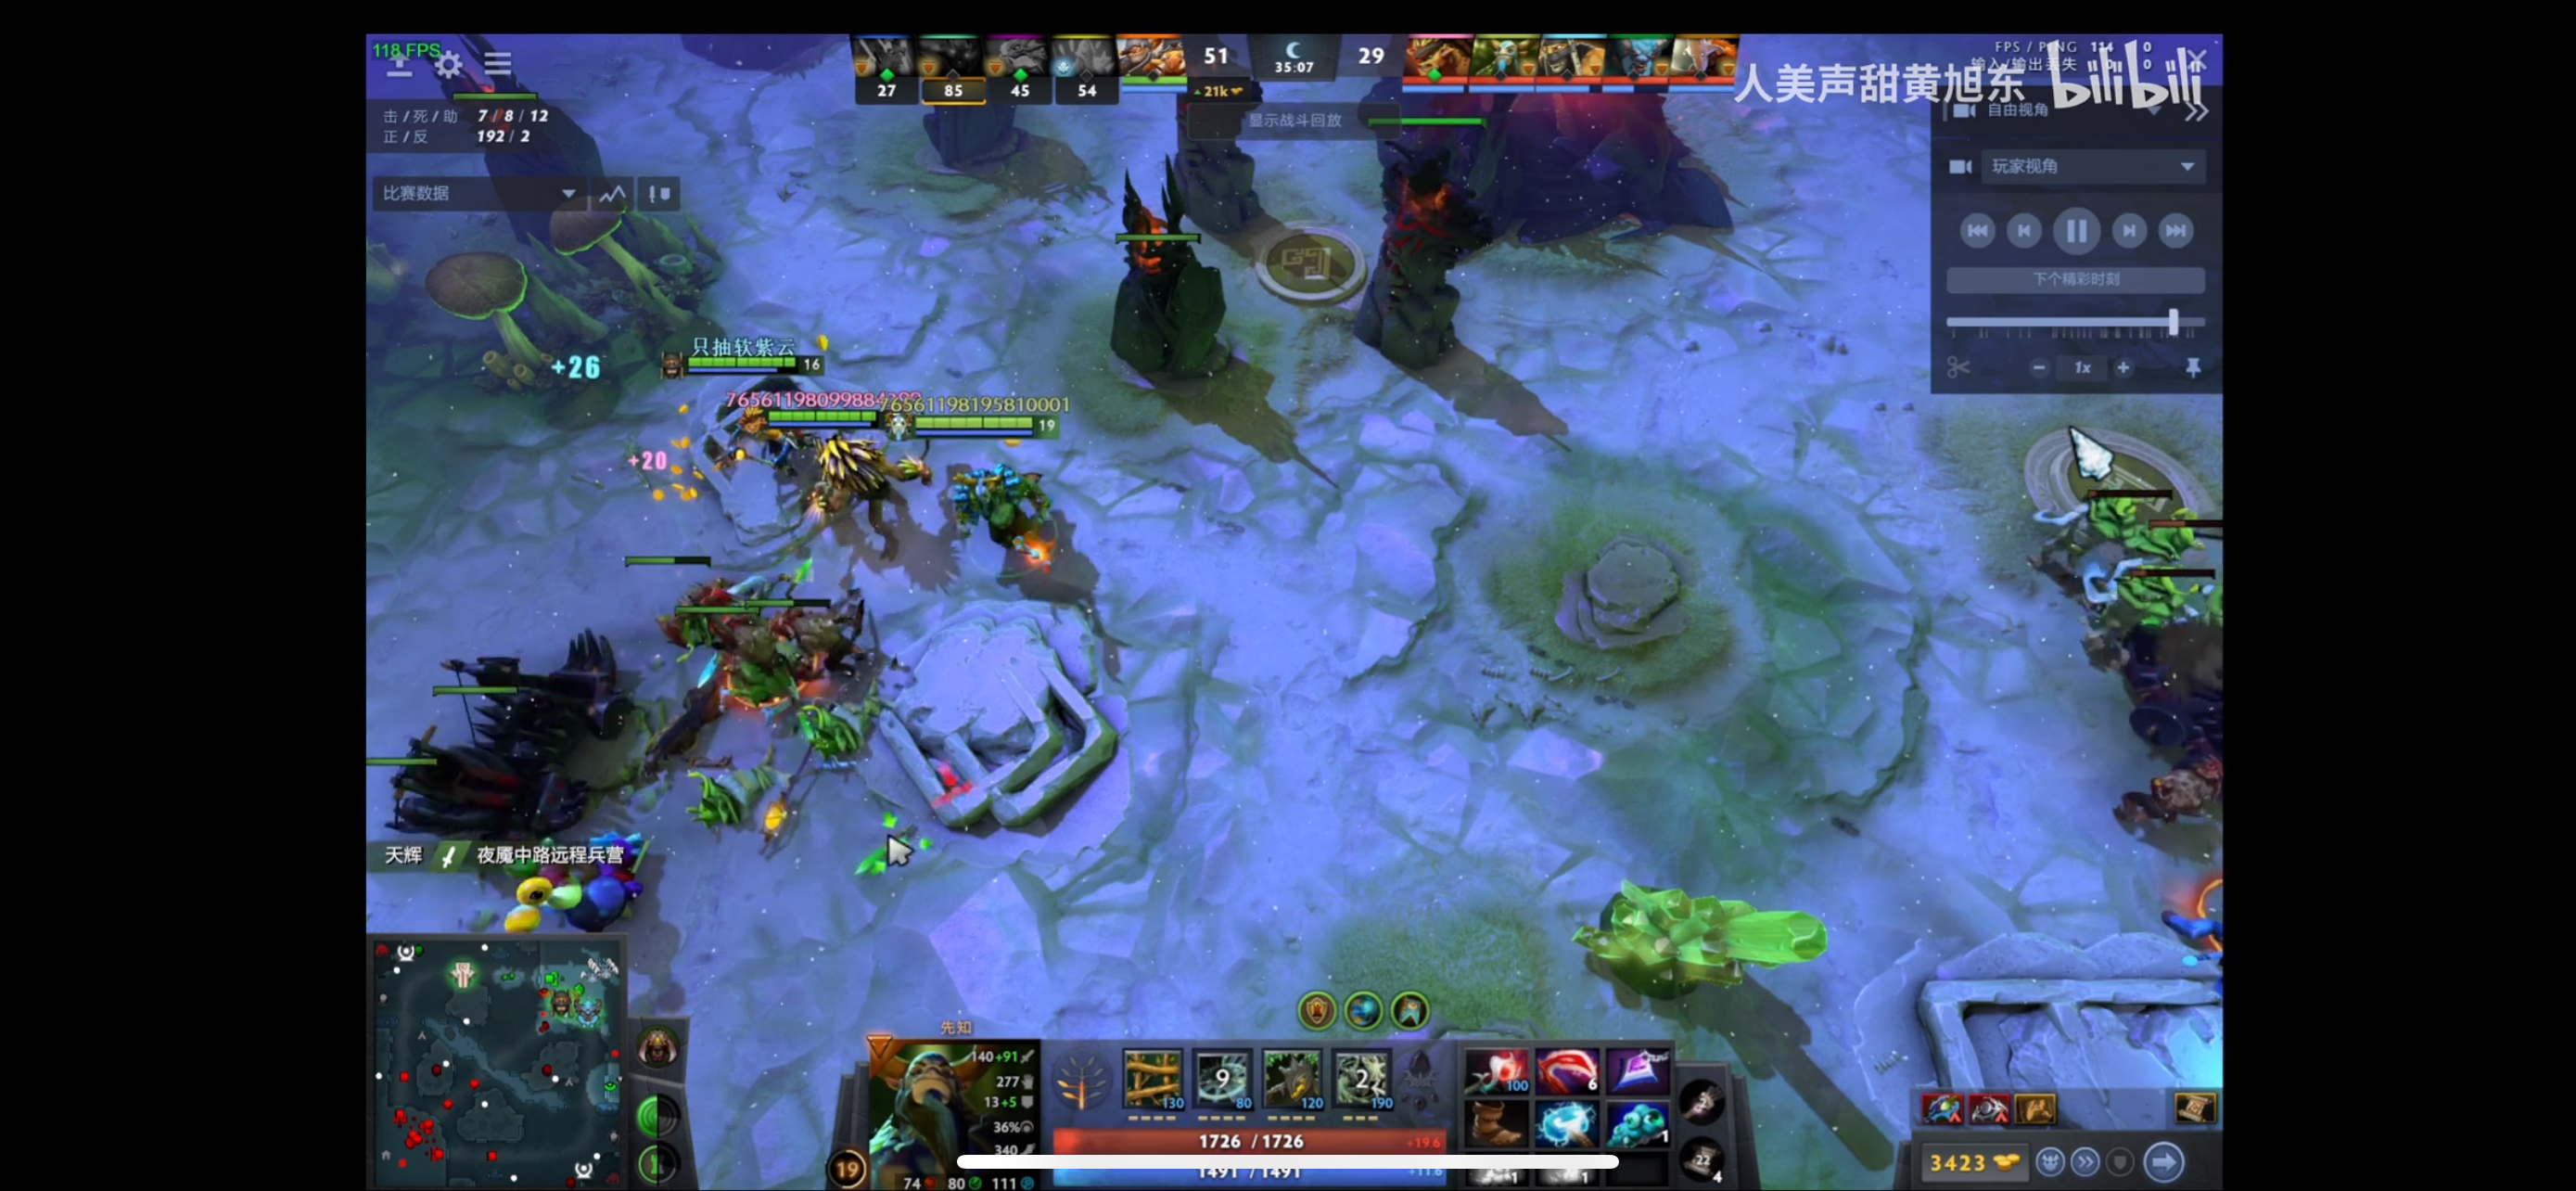
\includegraphics[width=\textwidth]{fig/3.png} % 图片3
        \caption{图3}
    \end{subfigure}

    \medskip % 垂直间距

    \begin{subfigure}{0.3\textwidth}
        \centering
        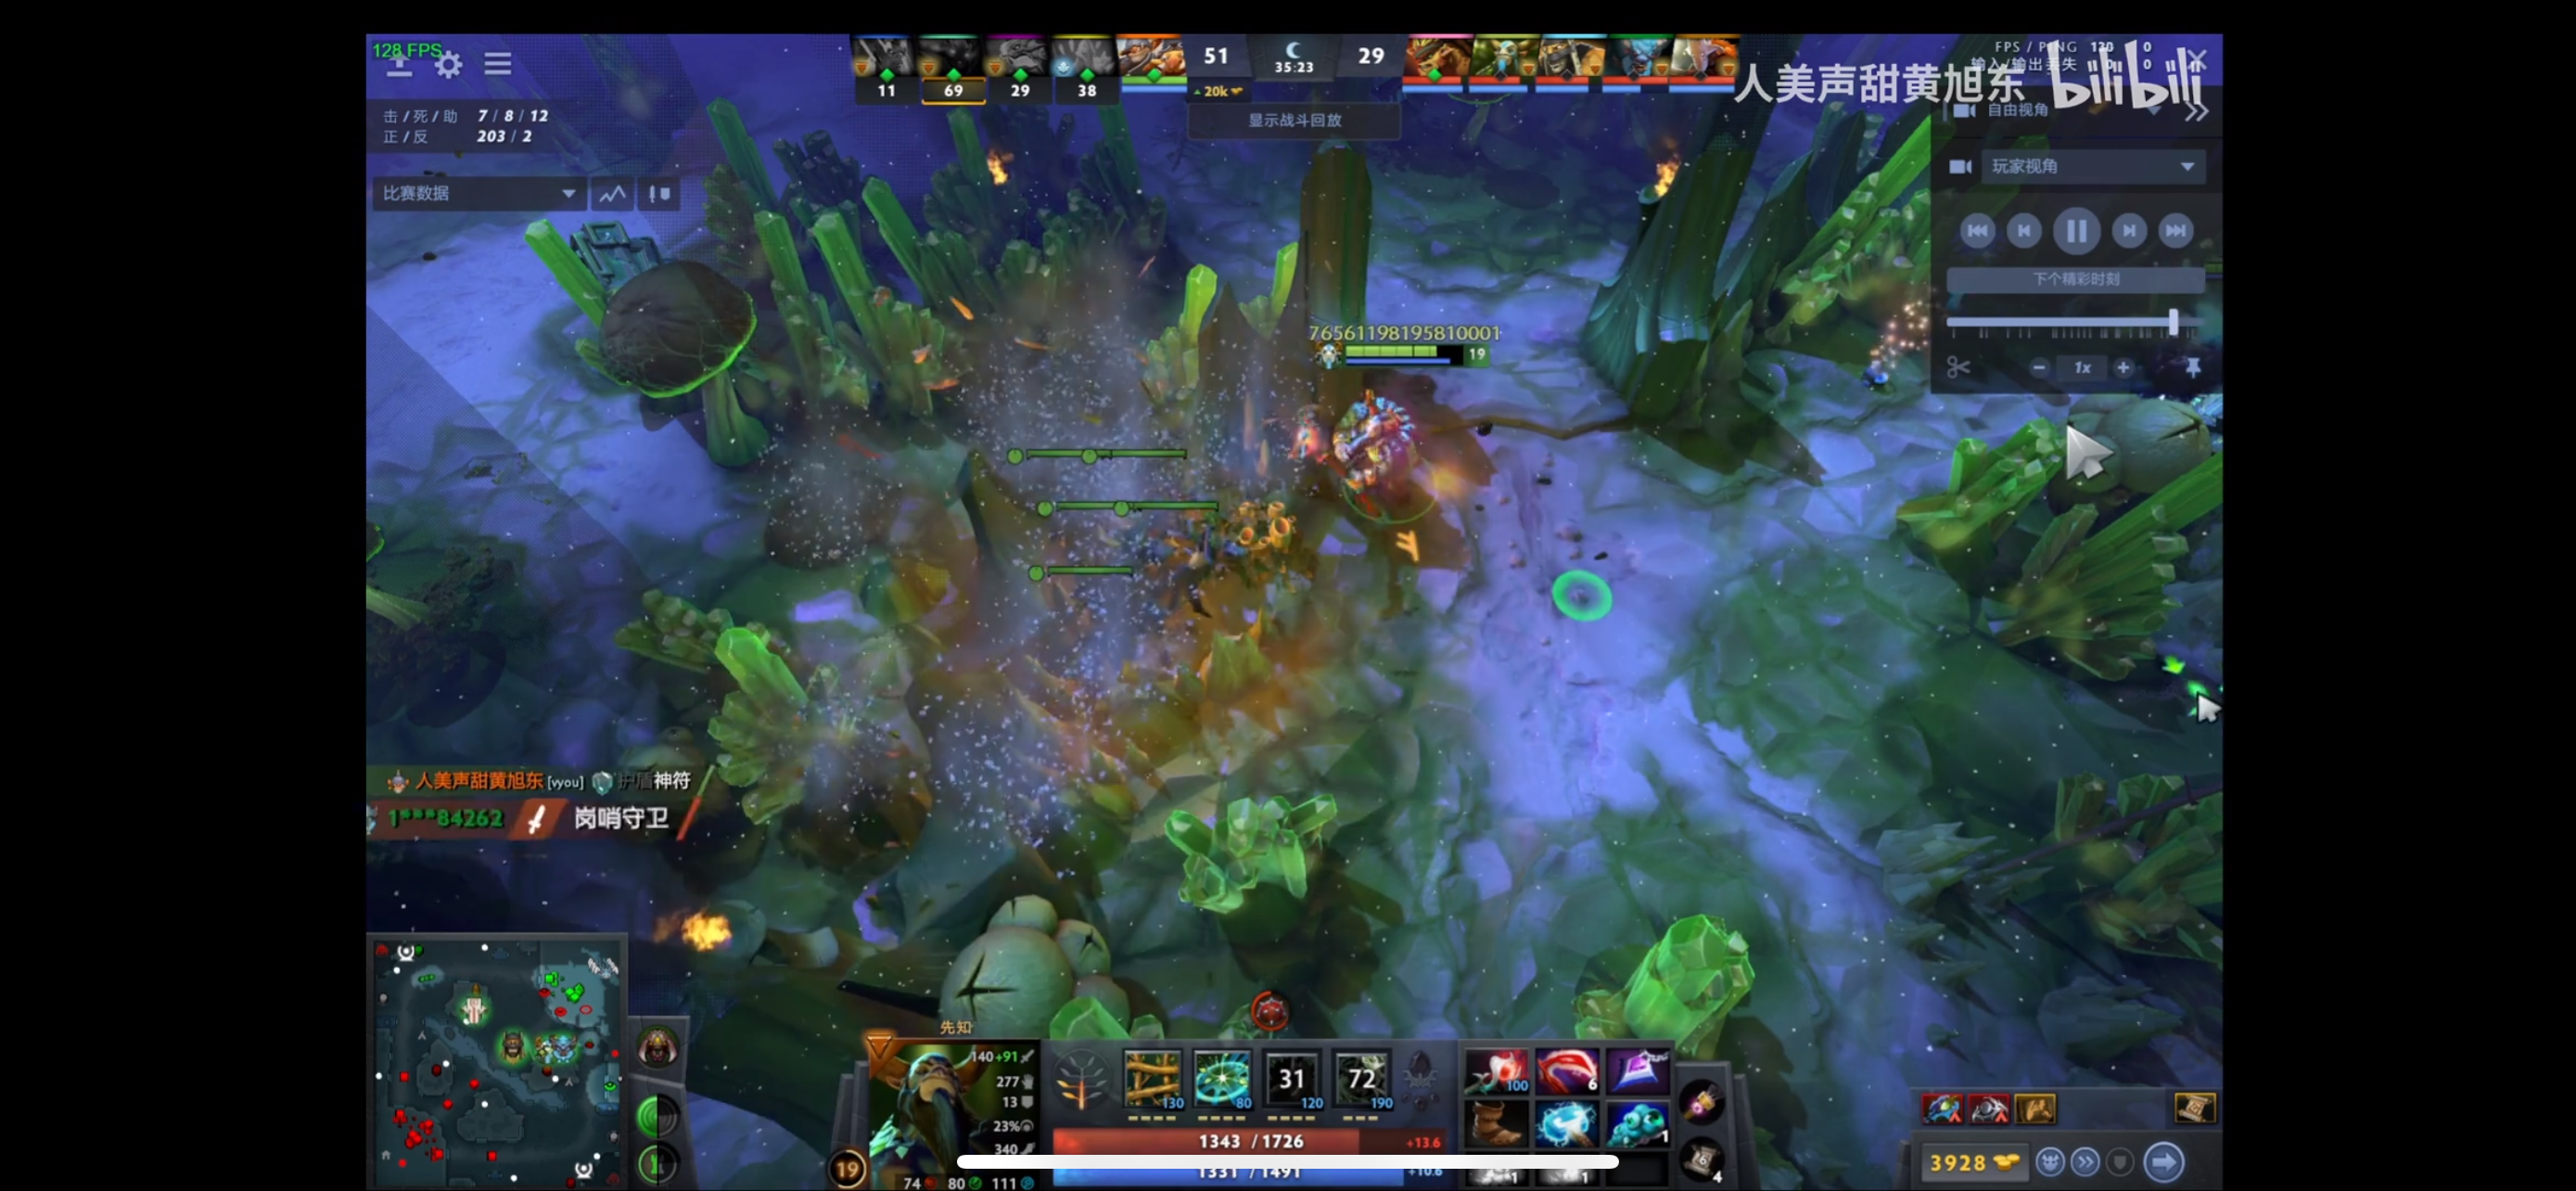
\includegraphics[width=\textwidth]{fig/4.png} % 图片4
        \caption{图4}
    \end{subfigure}
    \hfill
    \begin{subfigure}{0.3\textwidth}
        \centering
        \includegraphics[width=\textwidth]{fig/5.png} % 图片5
        \caption{图5}
    \end{subfigure}
    \hfill
    \begin{subfigure}{0.3\textwidth}
        \centering
        \includegraphics[width=\textwidth]{fig/6.png} % 图片6
        \caption{图6}
    \end{subfigure}

    \medskip % 垂直间距

    \begin{subfigure}{0.3\textwidth}
        \centering
        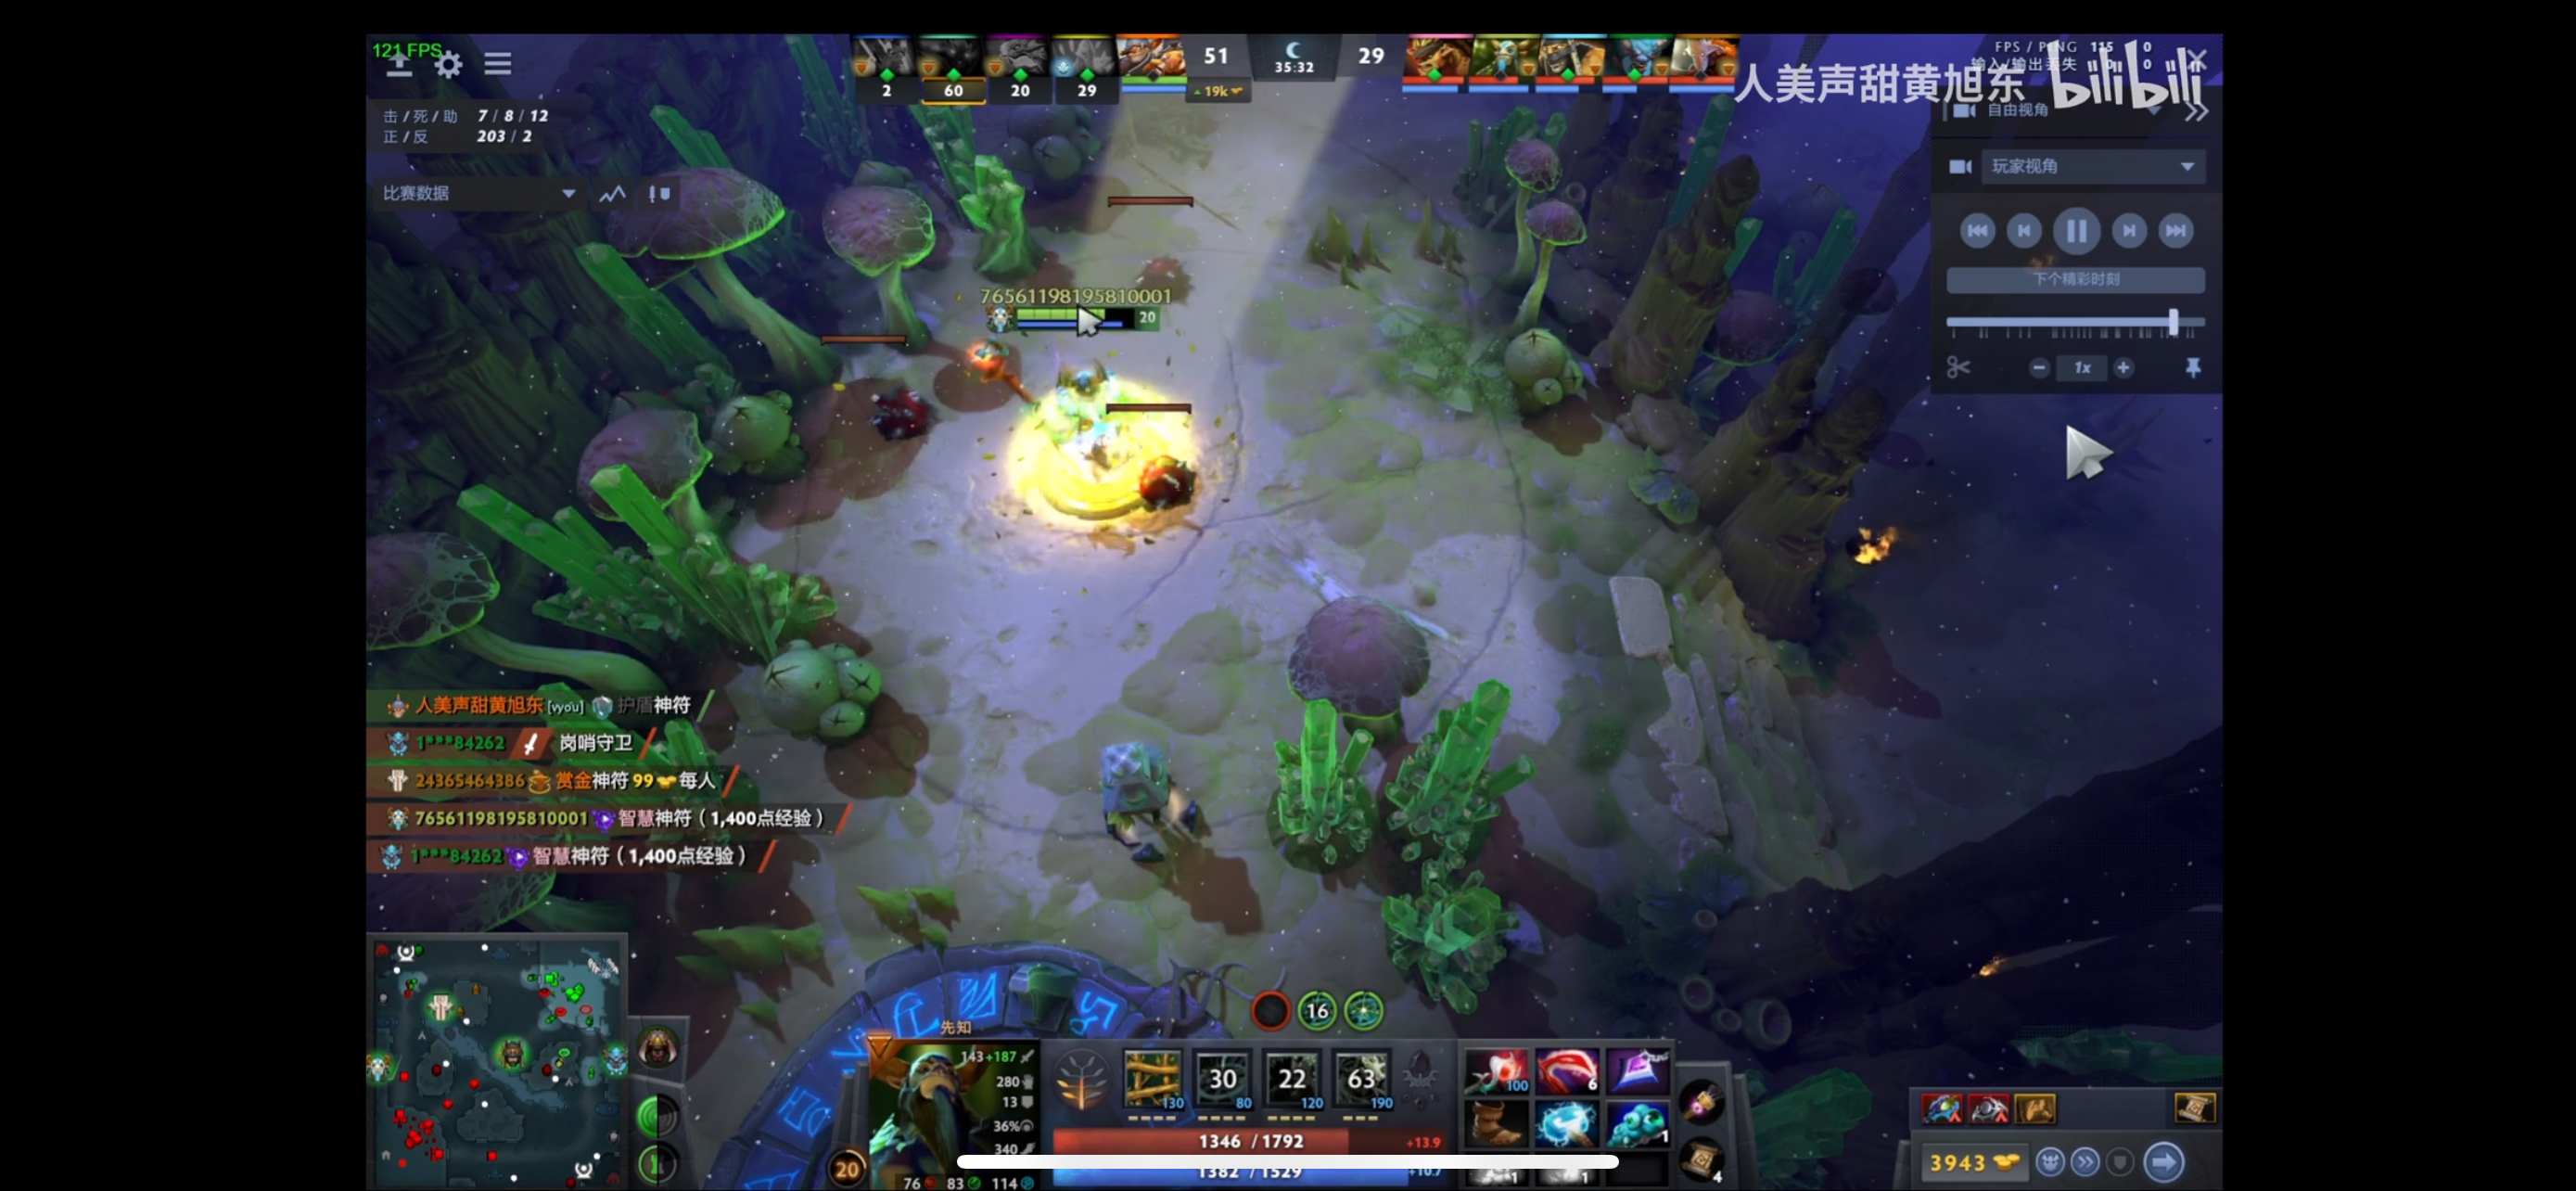
\includegraphics[width=\textwidth]{fig/7.png} % 图片7
        \caption{图7}
    \end{subfigure}
    \hfill
    \begin{subfigure}{0.3\textwidth}
        \centering
        
\includegraphics[width=\textwidth]{fig/8.png} % 图片8
        \caption{图8}
    \end{subfigure}
    \hfill
    \begin{subfigure}{0.3\textwidth}
        \centering
        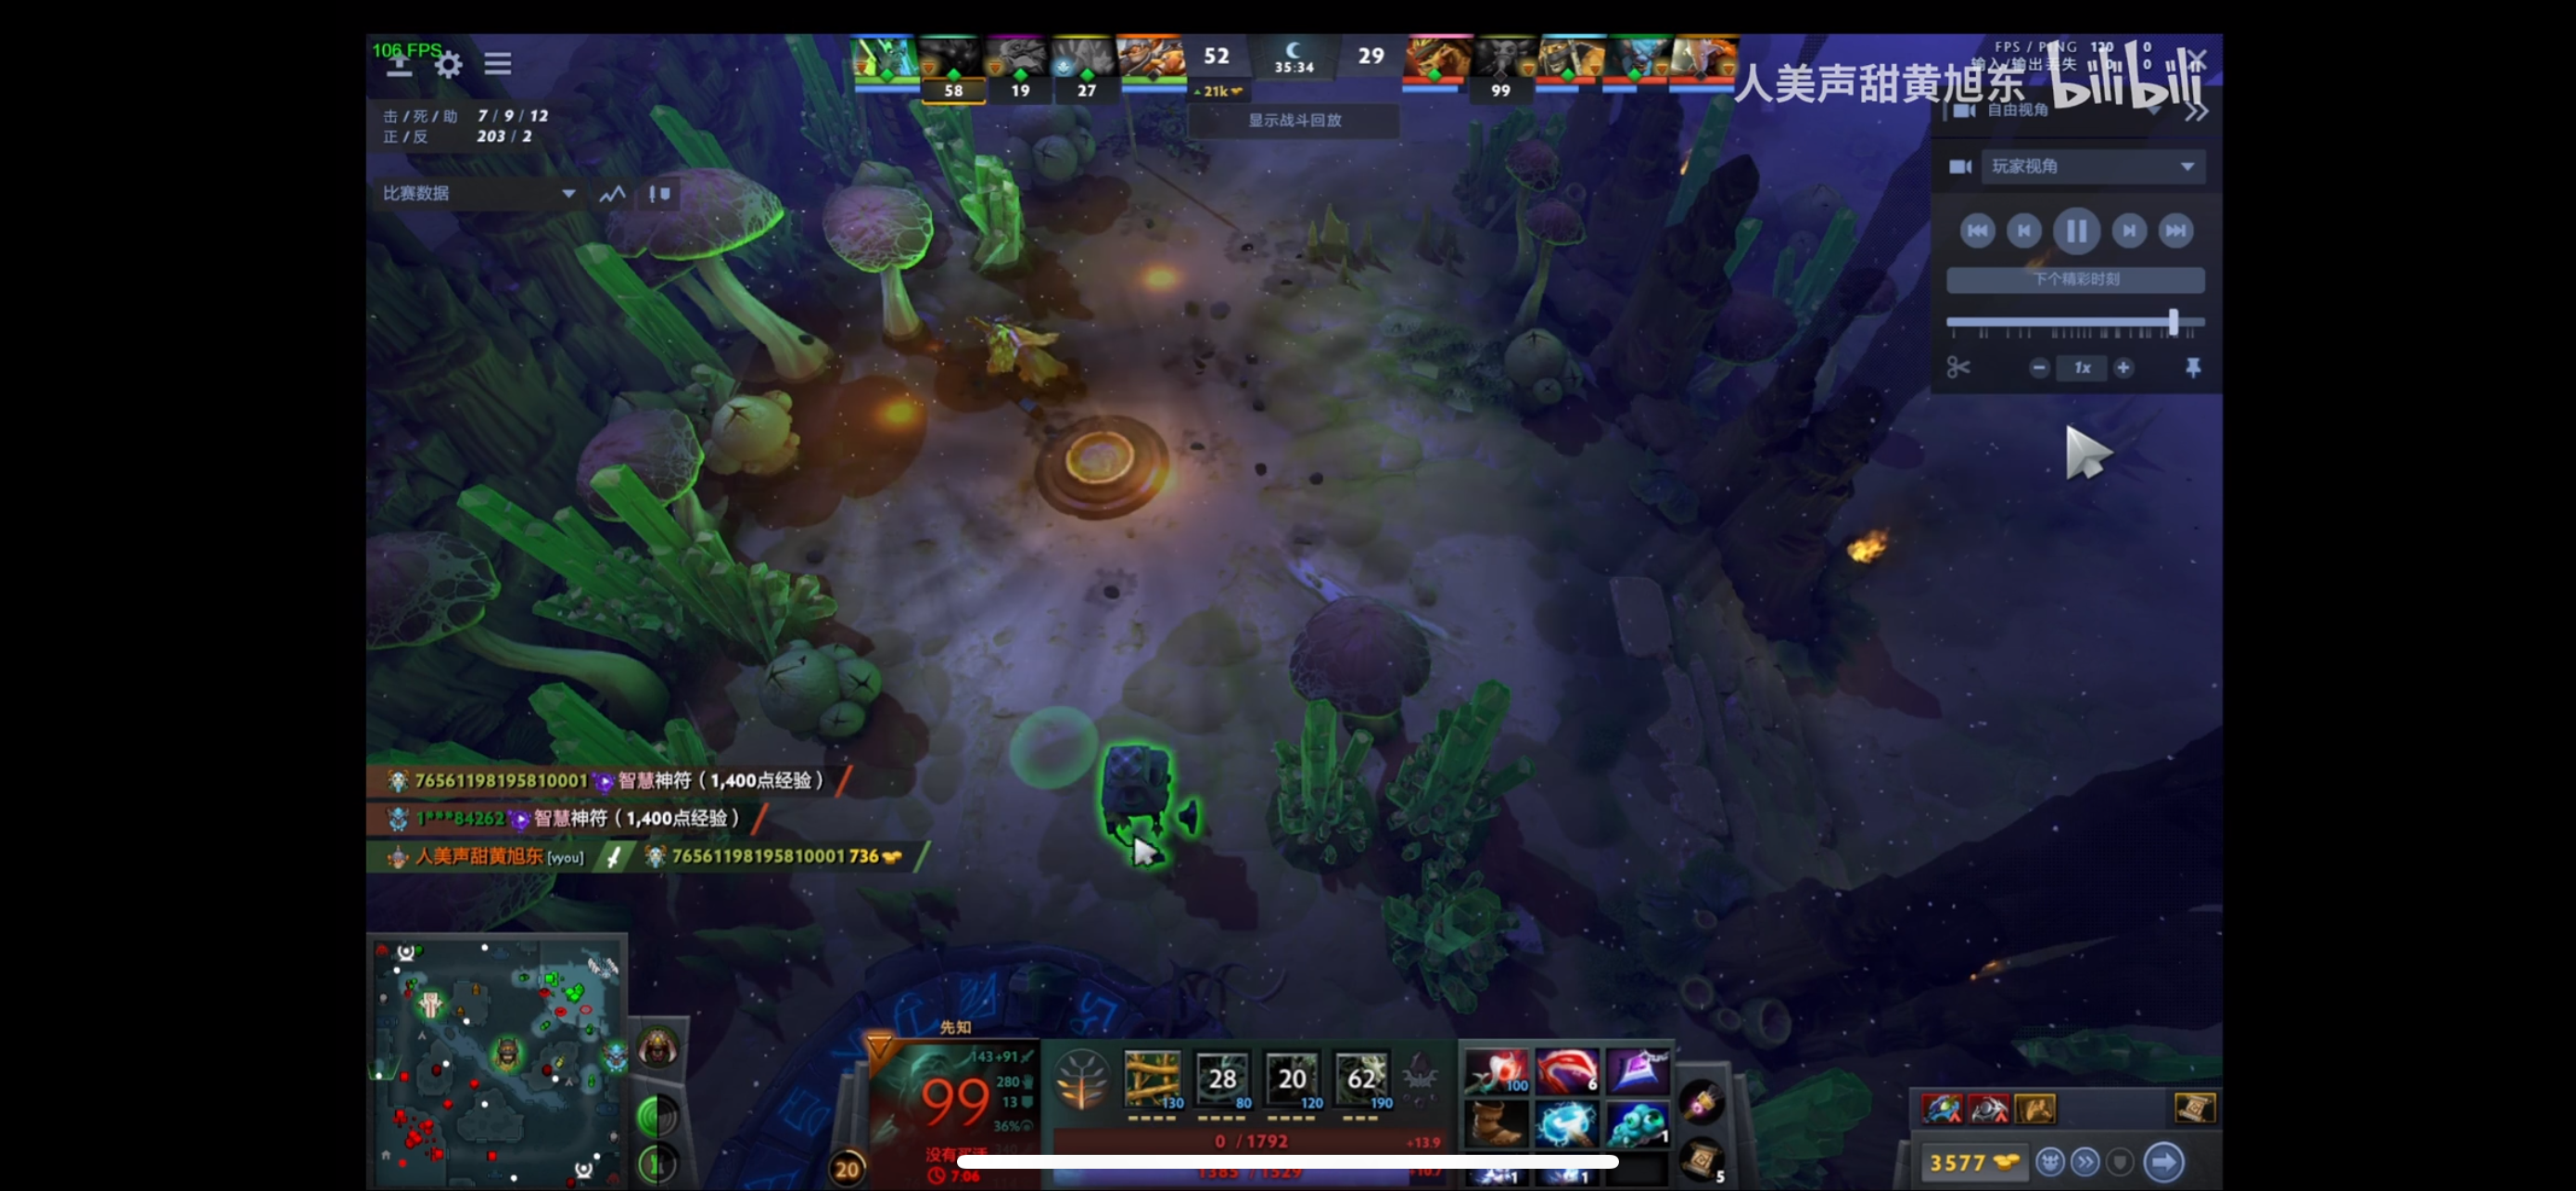
\includegraphics[width=\textwidth]{fig/9.png} % 图片9
        \caption{图9}
    \end{subfigure}

    \caption{九宫格图片布局}
\end{figure}

\newpage

\section{公式}
\textbf{希腊字母}:
\vspace{2mm} \\
\begin{tabular}{|l|l|l|l|l|l|}
    \hline
    $ \alpha $ & \verb|\alpha|  & $ \beta $    & \verb|\beta|    & $ \gamma $      & \verb|\gamma|      \\ \hline
    $ \delta $ & \verb|\delta|  & $ \epsilon $ & \verb|\epsilon| & $ \varepsilon $ & \verb|\varepsilon| \\ \hline
    $ \zeta  $ & \verb|\zeta|   & $ \eta $     & \verb|\eta|     & $ \theta $      & \verb|\theta|      \\ \hline
    $ \lambda$ & \verb|\lambda| & $ \mu  $     & \verb|\mu|      & $ \nu $         & \verb|\nu|         \\ \hline
    $ \xi    $ & \verb|\xi|     & $ \pi $      & \verb|\pi|      & $ \rho $        & \verb|\rho|        \\ \hline
    $ \sigma $ & \verb|\sigma|  & $ \tau $     & \verb|\tau|     & $ \phi $        & \verb|\phi|        \\ \hline
    $ \varphi$ & \verb|\varphi| & $ \psi $     & \verb|\psi|     & $ \omega $      & \verb|\omega|      \\ \hline
\end{tabular}
\vspace{2mm}  \\
以下字母存在大写形式(省略了一些带\verb|\var|前缀的),只需把首字母大写即可。

\subsection{单行公式}
单行公式较为简单,直接在\$...\$之间输入公式代码即可,例如:\par
\begin{equation}
    E_0=mc^2
\end{equation}

\subsection{多行公式}
多行公式涉及到手动在恰当的地方用$\backslash$$\backslash$分行,
同时用\&对齐,本模板中以等号对齐为例:\\
\begin{equation}
    \begin{split}
        Dec_{sk}(\alpha)&=(a_1\cdot a_2)+(a_2\cdot b_1)+(a_1\cdot b_2)\\
        &= m_1m_2-m_1b_2-m_2b_1+b_1b_2+m_2b_1-b_1b_2+m_1b_2-b_1b_2\\
        &= m_1m_2-b_1b_2
    \end{split}
\end{equation}
\subsection{分情况讨论}

$$
    \begin{cases}
        \Delta >0 & \text{方程有两个不相等的实根} \\
        \Delta =0 & \text{方程有两个相等的实根}  \\
        \Delta <0 & \text{方程有两个复根}     \\
    \end{cases}
$$
\subsection{公式编号}
还没想好捏

\section{算法}

\begin{algorithm}
    \renewcommand{\algorithmicrequire}{\textbf{Input:}}
    \renewcommand{\algorithmicensure}{\textbf{Output:}}
    \caption{斐波那契数列算法}
    \label{alg:fibonacci}
    \begin{algorithmic}[1]
        \REQUIRE  斐波那契数列的长度$n$
        \ENSURE 斐波那契数列的前$n$项
        \STATE Initialize $F[0] \gets 0$, $F[1] \gets 1$
        \FOR{$i = 2$ to $n$}
        \STATE $F[i] \gets F[i-1] + F[i-2]$
        \ENDFOR
        \STATE \textbf{return} 斐波那契数列 $F[0], F[1], \ldots, F[n-1]$
    \end{algorithmic}
\end{algorithm}


\newpage

\printbibliography[title=参考文献]

\begin{appendices}
    \renewcommand{\thesection}{\Alph{section}}
    \section{附录标题}
    这里是附录.
\end{appendices}

\end{document}